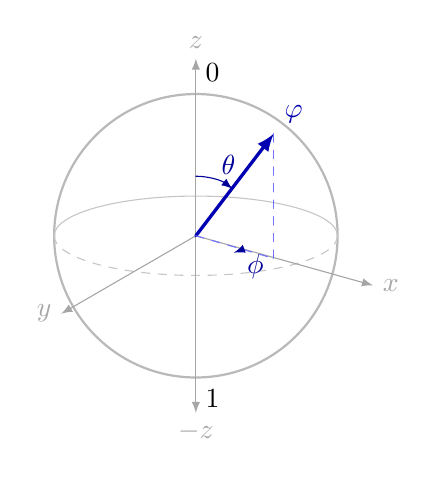
\begin{tikzpicture}[
  scale=1.8,
  line cap=round,
  line join=round,
  >=latex
]
  % ===== theta と phi を調整する場所 =====
  % 状態ベクトル |varphi> の先端です。
  % theta や phi を大きく変えるときは、この点も一緒に動かします。
  \coordinate (varphi) at (0.55,0.72);

  % 状態ベクトルを赤道面に下ろした点です。
  % phi を変えるときは、この点を赤道上で左右に動かします。
  \coordinate (varphiProjection) at (0.55,-0.16);

  % theta の弧の終点角度です。
  % 90度が z軸方向で、値を小さくすると |varphi> が右側へ倒れます。
  \def\ThetaEndAngle{52}

  % phi の弧の始点・終点角度です。
  % 今は -16度から -37度まで描いています。
  % phi を大きく見せたいときは \PhiEndAngle をさらに小さくします。
  \def\PhiStartAngle{-16}
  \def\PhiEndAngle{-37}

  % 球体
  \draw[gray!55, thick] (0,0) circle (1);
  \draw[gray!45, dashed] (-1,0) arc[start angle=180, end angle=360, x radius=1, y radius=0.28];
  \draw[gray!45] (1,0) arc[start angle=0, end angle=180, x radius=1, y radius=0.28];

  % 座標軸
  \draw[->, gray!70] (0,0) -- (0,1.25) node[above] {$z$};
  \draw[->, gray!70] (0,0) -- (0,-1.25) node[below] {$-z$};
  \draw[->, gray!70] (0,0) -- (1.25,-0.35) node[right] {$x$};
  \draw[->, gray!70] (0,0) -- (-0.95,-0.55) node[left] {$y$};

  % 基底状態
  \node[above right] at (0,1.02) {$\ket{0}$};
  \node[below right] at (0,-1.02) {$\ket{1}$};

  % 量子状態
  \draw[very thick, blue!70!black, ->] (0,0) -- (varphi) node[above right] {$\ket{\varphi}$};

  % 点線
  \draw[blue!55, dashed] (varphi) -- (varphiProjection);
  \draw[blue!55, dashed] (0,0) -- (varphiProjection);

  % 角度
  \draw[->, blue!60!black] (0,0.42) arc[start angle=90, end angle=\ThetaEndAngle, radius=0.42];
  \node[blue!60!black] at (0.23,0.50) {$\theta$};

  \draw[->, blue!60!black] (0.32,-0.09) arc[start angle=\PhiStartAngle, end angle=\PhiEndAngle, x radius=0.32, y radius=0.09];
  \node[blue!60!black] at (0.42,-0.22) {$\phi$};
\end{tikzpicture}
